\subsection{包络代数的滤子}

设 g 是 K 上的李代数，T 是 K-模 g 的张量代数。令 \(T^{n}\) 为 T 中由 n 阶齐次张量组成的子模

并令 \(\mathrm{T_n} = \sum_{i\leqslant n}\mathrm{T^i}\)。则 \(\mathrm{T_n}\subset \mathrm{T}_{n + 1},\mathrm{T_0} = \mathrm{K}.1,\mathrm{T}_{-1} = \{0\}\)，且 \(\mathrm{T_nT_p}\subset \mathrm{T}_{n + p}\)。令 \(\mathbf{U}_n\) 为 \(\mathbf{T}_n\) 在 g 的包络代数 U 中的典范像。则 \(\mathrm{U_n}\subset \mathrm{U}_{n + 1},\mathrm{U_0} = \mathrm{K}.1,\mathrm{U}_{-1} = \{0\}\)，且 \(\mathrm{U_nU_p}\subset \mathrm{U}_{n + p}\)；因此 U 可描述为由 \(\mathbf{U}_n\) 滤过的代数（Commutative Algebra, Chapter III, §2, no. I）；\(\mathrm{U_n}\) 中的元素称为滤子次数 \(\leqslant n\) 的元素。

令 \(G^n\) 为 K-模 \(U_n / U_{n-1}\)，令 G 为各 \(G^n\) 的直和这个 K-模。U 上的乘法在取商后定义了从 \(G^n \times G^m\) 到 \(G^{n+m}\) 的双线性映射，因而定义了从 \(G \times G\) 到 G 的双线性映射，该映射是结合的。于是 G 具有结合 K-代数结构。并且 \(G^n G^m \subset G^{n+m}\)。\(G^n\) 的元素称为 n 次元素。如此得到的分次代数正是滤过代数 U 的关联分次代数（Commutative Algebra, Chapter III, § 2, no. 3）。

令 \(\phi_{n}\) 为下列典范 K-线性映射的复合

\[
\mathrm{T} ^ {n} \rightarrow \mathrm{U} _ {n} \rightarrow \mathrm{G} ^ {n}.
\]

由于 \(\mathbf{T}^n\) 是 \(\mathbf{T}_{n - 1}\) 在 \(\mathbf{T}_n\) 中的补空间，\(\phi_n\) 是满射。各 \(\phi_n\) 定义了 K-线性满射 \(\phi\)，它从 \(\sum_{n}\mathbf{T}^{n} = \mathbf{T}\) 到 \(\sum_{n}\mathbf{G}^{n} = \mathbf{G}\)。

命题 5. 从 T 到 G 的映射 \(\phi\) 是将 1 映到 1 的代数同态，并且在由张量 \(x \otimes y - y \otimes x\)（\(x \in \mathfrak{g}, y \in \mathfrak{g}\)）生成的双边理想上为零。

若 \(t \in \mathbf{T}^n\) 且 \(t' \in \mathbf{T}^p\)，则按乘法定义，有 \(\phi(t)\phi(t') = \phi(tt')\)，其中乘法定义在 \(\mathbf{G}\) 上。所以 \(\phi\) 是代数同态，且显然 \(\phi(1) = 1\)。若 \(x, y\) 属于 \(\mathfrak{g}\)，则 \(x \otimes y - y \otimes x \in \mathbf{T}^2\)，且此元素在 \(\mathrm{U}_2\) 中的典范像等于 \([x, y]\) 的典范像，因而属于 \(\mathrm{U}_1\)。所以 \(\phi(x \otimes y - y \otimes x) = 0\)，命题得证。

令 S 为 K-模 g 的对称代数，\(\tau\) 为从 T 到 S 的典范同态。命题 5 表明，存在唯一的将 1 映到 1 的从代数 S 到代数 G 的同态 \(\omega\)，称为典范同态，使 \(\phi = \omega \circ \tau\)。有 \(\omega(\mathrm{S}^{n}) = \phi(\mathrm{T}^{n}) = \mathrm{G}^{n}\)。令 \(\tau_{n}\) 为 \(\tau\) 在 \(T^{n}\) 上的限制，\(\omega_{n}\) 为 \(\omega\) 在 \(S^{n}\) 上的限制，\(\psi_{n}\) 为从 \(T^{n}\) 到 \(U_{n}\) 的典范映射，\(\theta_{n}\) 为从 \(U_{n}\) 到 \(G^{n}\) 的典范映射。由 \(\omega_{n}\) 的定义，下图交换：

\pandocbounded{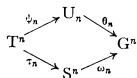
\includegraphics[keepaspectratio]{images/part001_82008693.jpg}}

命题 6. 若 K 是 Noetherian 环且 g 是有限生成模，则环 U 是左、右 Noetherian 的。

S 是 K 上的有限生成代数，因而是 Noetherian 环（Commutative Algebra, Chapter III, § 2, no. 10, Corollary 3 to Theorem 2）。所以，与 S 的商环同构的 G 是 Noetherian 的。因此 U 是左、右 Noetherian 的（Commutative Algebra, Chapter III, § 2, no. 10, Remark 2）。

推论. 设 K 是域，g 是 K 上的有限维空间。令 \(I_{1}, \ldots, I_{m}\) 为 U 中有限余维的右（分别为左）理想。则积理想 \(I_{1}I_{2}\ldots I_{m}\) 具有有限余维。

对 m 归纳，只需考虑例如两个右理想的情形。右 U-模 \(I_{1}\) 由有限个元素 \(u_{1},\ldots,u_{p}\) 生成（命题 6）。令 \(v_{1},\ldots,v_{q}\) 为 U 中的元素，使其模 \(I_{2}\) 的类生成向量空间 \(U/I_{2}\)。于是，\(I_{1}/I_{1}I_{2}\) 中 \(u_{i}v_{j}\) 的典范像生成向量空间 \(I_{1}/I_{1}I_{2}\)，该空间因而是有限维的。所以 \(\dim_{\mathbb{K}}(\mathrm{U}/\mathrm{I}_{1}\mathrm{I}_{2})=\dim_{\mathbb{K}}(\mathrm{U}/\mathrm{I}_{1})+\dim_{\mathbb{K}}(\mathrm{I}_{1}/\mathrm{I}_{1}\mathrm{I}_{2})<+\infty\)。

注. 设 \(g'\) 是环 K 上的另一个李代数，\(U'\) 是其包络代数，\(U_n'\) 是 \(U'\) 中滤子次数 \(\leqslant n\) 的元素的集合，\(U^n\)（分别为 \(U'^n\)）是 U（分别为 \(U'\)）中 g（分别为 \(g'\)）的 n 阶齐次对称张量的典范像的集合。令 \(\eta\) 为从 g 到 \(g'\) 的同态，\(\tilde{\eta}\) 为相应的从 U 到 \(U'\) 的同态。则

\[
\tilde {\eta} (\mathrm{U} _ {n}) \subset \mathrm{U} _ {n} ^ {\prime}, \quad \tilde {\eta} (\mathrm{U} ^ {n}) \subset \mathrm{U} ^ {\prime n}.
\]

特别地，U 的主反自同构保持 \(U_{n}\) 和 \(U^{n}\) 稳定。将 \(T^{n}\) 映到自身的 K-线性映射为：

\[
x _ {1} \otimes x _ {2} \otimes \dots \otimes x _ {n} \quad \text { to } \quad x _ {n} \otimes x _ {n - 1} \otimes \dots \otimes x _ {1}
\]

对 g 中所有 \(x_{1},\ldots,x_{n}\) 的映射是一个对称算子，因而保持 n 阶齐次对称张量不变。因此，U 的主反自同构在每个 \(U^{n}\) 上诱导出比为 \((-1)^{n}\) 的伸缩变换。

